\documentclass[border=2pt]{standalone}
\usepackage{tikz}
\usetikzlibrary{quotes,angles}
\usepackage{amsmath}
\usepackage{amssymb}

\begin{document}

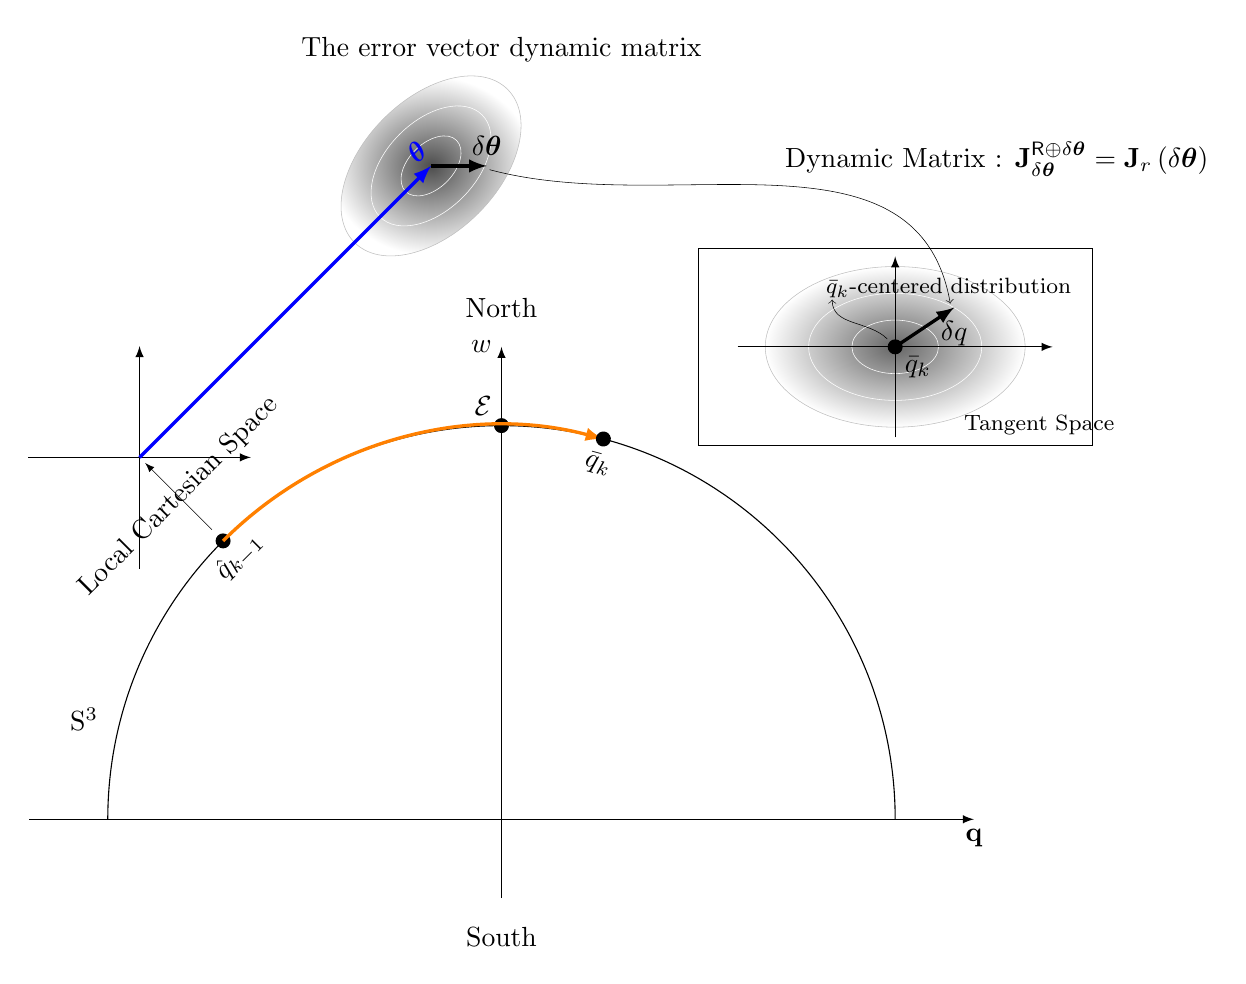
\begin{tikzpicture}[scale=5]

% Draw x and y axis lines
\draw [->,>=latex] (-1.2,0) -- (1.2,0) node [below] {$\mathbf{q}$};
\draw [->,>=latex] (0,-0.2) -- (0,1.2) node [left] {$w$};
\node [above] at (0, 1.25) {North};
\node [below] at (0,-0.25) {South};
\node[above left] at (-1.0,0.2) {$\mathrm{S}^{3}$};
\node[above] at (0.0,1.9) {The error vector dynamic matrix};

% Draw a arc at the origin of radius 1
\draw (1,0) arc (000:180:1);
\filldraw[black] (0,1) circle (0.5pt) node[above left ] {$\mathcal{E}$} ;

\begin{scope} [rotate=45]

\filldraw[black] (0.0,1.0) circle (0.5pt) node[below, rotate=45 ] {$\hat{q}_{k-1}$} ;
%\draw [very thin] (-.5, 1) -- ( 1.1, 1) node[right, rotate=45] {Tangent Space} ;
%\draw [very thick, ->, >=latex, blue] (0,1) -- (1.047,1) node[above , rotate=45] {$\left[0, \boldsymbol{\theta}\right]$} ;

\draw [->,>=latex] [very thick, orange] (0,1) arc (90:30:1);

% 0.8660 , 0.5000
%\draw [->,>=latex] [very thin] (1.047,0.98) to [out=270,in=30] (0.88,0.51) ;
%\node [fill=white, rotate=45] at (1.05,0.75) {\footnotesize$\mathrm{Exp}\left( \color{blue}\boldsymbol{\theta}\color{black} \right)$} ;

%\node[above, rotate=45] at (0.0,1.4) {$\hat{\boldsymbol{P}}_{k-1}$};
\begin{scope} [shift={(0.0,1.3)}]
\draw [->,>=latex] (-0.2, 0.2) -- ( 0.2,-0.2) ;
\draw [->,>=latex] (-0.2,-0.2) -- ( 0.2, 0.2) ;
\end{scope}
\draw [very thin, ->,>=latex] (0.0, 1.04) -- node[ rotate=45] {Local Cartesian Space} ( 0.0, 1.28) ;

\begin{scope} [shift={(1.047, 1.3)}, scale=0.25]

% FIXME: 程序有BUG,旋转之后灰度边缘不对。
\draw [very thin, lightgray, inner color=black!70, outer color=black!0] (0,0) ellipse (1.1 and 0.68);
\draw [very thin, lightgray!0] (0,0) ellipse (1.1/3*2 and 0.68/3*2); % \sigma = +-2
\draw [very thin, lightgray!0] (0,0) ellipse (1.1/3   and 0.68/3  ); % \sigma = +-1

\end{scope}

%\node[above, rotate=45] at (1.047,1.4) {$\bar{\boldsymbol{P}}_{k}$};

\draw [very thick, ->,>=latex, color=blue] (0.0, 1.3) -- (1.047, 1.3) node[above , rotate=45] {$\boldsymbol{\theta}$} ;
\begin{scope} [shift={(1.047, 1.3)}]
\draw [very thick, ->,>=latex] ( 0.0, 0.0) -- ( 0.1,-0.1) node[above] {$\delta\boldsymbol{\theta}$} ;
\end{scope}

\end{scope}

\begin{scope} [rotate=-15]

\filldraw[black] (0.0,1.0) circle (0.5pt) node[below=2pt, rotate=-15 ] {$\bar{q}_{k}$} ;

\end{scope}

\begin{scope} [shift={(1.0, 1.2)}]

\draw [very thin] (-0.5,-0.25) rectangle (0.5,0.25);
%\draw [very thin] (-0.60,-0.30) rectangle ( 0.60, 0.30);

\begin{scope} [scale=0.30]

% FIXME: 程序有BUG,旋转之后灰度边缘不对。
\draw [very thin, lightgray, inner color=black!60, outer color=black!0] (0,0) ellipse (1.1 and 0.68);
\draw [very thin, lightgray!0] (0,0) ellipse (1.1/3*2 and 0.68/3*2); % \sigma = +-2
\draw [very thin, lightgray!0] (0,0) ellipse (1.1/3   and 0.68/3  ); % \sigma = +-1

\end{scope}

\draw [->,>=latex] (-0.4, 0.00) -- ( 0.4, 0.00) ;
\draw [->,>=latex] ( 0.0,-0.23) -- ( 0.0, 0.23) ;

\filldraw[black] ( 0.0, 0.0) circle (0.5pt) node [below right] {$\bar{q}_{k}$};
%\filldraw[black] ( 0.1, 0.1) circle (0.5pt) node [below right] {$\delta q$};
\draw [very thick, ->,>=latex] ( 0.0, 0.0) -- ( 0.15, 0.1) node[below=1pt ] {$\delta q$} ;

\node [below right] at (-0.20, 0.20) {\footnotesize $\bar{q}_{k}$-centered distribution};
\node [below right] at ( 0.15,-0.15) {\footnotesize Tangent Space};

\draw [very thin, ->] (-0.02, 0.02) to [out=135,in=-90] (-0.16, 0.12) ;

\end{scope}

\draw [very thin, ->] (-0.03, 1.65) to [out=-15,in=100] node[above right] {Dynamic Matrix : $\mathbf{J}_{\delta\boldsymbol{\theta}}^{\mathsf{R}\oplus\delta\boldsymbol{\theta}}=\mathbf{J}_{r}\left(\delta\boldsymbol{\theta}\right)$} (1.14, 1.31) ;

\end{tikzpicture}

\end{document}

